The transmitter is the part that provides to convert the received sounds signals in commands for the robot, through a microphone. The STM32D407VG-Discovery board is equipped with a MP45DT02 MEMS microphone and a CS43L22 DAC for audio acquisition and processing. In this project, these devices are used to detect the sounds' frequency, which will determine the commands to give to the robot.

\subsection{The MP45DT02 microphone}
The MP45DT02-M is a compact, low-power, omnidirectional, digital MEMS (Micro Electro-Mechanical Systems) microphone.
\begin{figure}[H]
	\hspace*{0.15 \textwidth}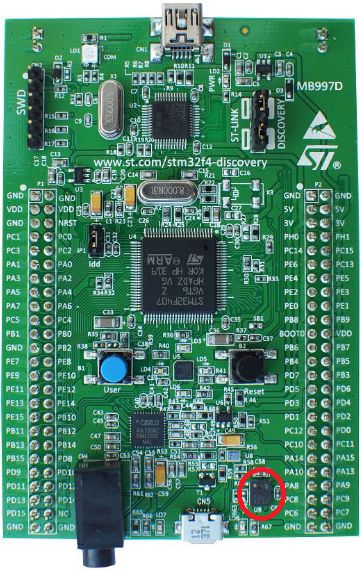
\includegraphics[width= 0.7\textwidth]
	{files/images/board_view}
	\caption{View of the upper surface of the board, with the microphone highlighted in the circle.}
\end{figure}

In the microphone bottom surface, there are six pins:
\begin{enumerate}
	\item \textbf{GND}: Connected to the GND of the board.
	\item \textbf{LR} - Channel selection: used since the microphone is designed to allow stereo audio capture. If it is connected to GND, the MP45DT02 is placed in \textit{left} channel mode: a sample is latched to the data output pin (PDM, Pulse-Density Modulation) on a falling edge of the clock, while on the rising clock edge, the output is set to high impedance. If the LR pin is connected to Vdd then the device operates in \textit{right} channel mode and the MP45DT02 latches it's sample to PDM on a clock rising edge, setting the pin to high impedance on the falling edge of the clock.
	\item \textbf{GND}: Connected to the GND of the board.
	\item \textbf{CLK} - Synchronization input clock: this pin is connected to the PB10 port of the board. The clock signal determines the sampling frequency.
	\item \textbf{DOUT} - PDM Data Output. Connected to the PC03 pin of the board's GPIO.
	\item \textbf{VDD}: Power supply.
\end{enumerate}

\begin{figure}[H]
	\hspace*{0.3 \textwidth}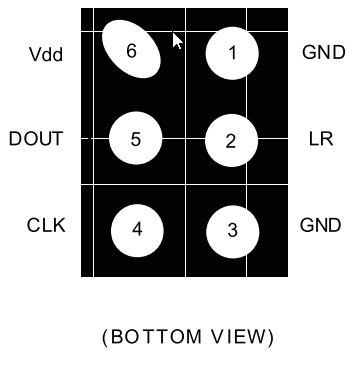
\includegraphics[width= 0.4\textwidth]
	{files/images/mic_bottom_pins}
	\caption{Pins on the bottom of the microphone.}
\end{figure}

\subsection{Overview on sound acquisition and processing}
The sound is acquired by the microphone, and the communication is performed through I2C.\\
The microphone acquires data in PDM format: each sample is a single bit, so the acquisition is a stream of bits; an high amplitude is represented with an high density of \textit{1} bits in the bitstream. \\
The sampling frequency of the ADC is 44000 Hz. \\
In order to process the data, it has to be converted in PCM (Pulse-Code Modulation) format: this is done by doing \textit{CIC filtering} (Cascaded Integrator-Comb), with a decimation factor of sixteen (each 16-bits sequence of 1-bit PDM samples is converted in one 16-bit PCM sample).\\
Then, an FFT (Fast Fourier Transform) analysis is performed on 4096 samples at a time to extract the fundamental frequency and the amplitude of the sound.

\subsubsection{Microphone initialization}
The initialization of the sound acquisition system comprehends several steps:
\begin{enumerate}
	\item SPI, DMA and General Purpose ports B and C are enabled through RCC
	\item GPIO ports are configured in \textit{Alternate} mode
	\item SPI is set to work in I2S mode
	\item Interrupt handling for DMA is configured
	
\end{enumerate}

\subsubsection{Sound acquisition and processing}
Each time a new block of samples is read, the \textit{freq\_recognition} library:
\begin{enumerate}
	\item Reads blocks of sixteen bits from SPI and transfers them in RAM through DMA;
	\item Converts 16 PDM samples in one 16-bit PCM sample via \textit{CIC filtering} with a decimation factor of sixteen;
	\item Perform FFT through the \textit{arm\_cfft\_radix4\_f32} module;
	\item Calculate amplitude of each frequency with the \textit{arm\_cmplx\_mag\_f32} module;
	\item Calculate the the fundamental frequency (and its amplitude) in the vector;
	\item Store the values of the fundamental frequency and its amplitude in dedicated variables, then ivoke the \textit{callback function} to react to the detected frequency.
\end{enumerate}
In this project, the \textit{callback function} is in charge of producing commands to the engines when the frequency of the last acquired sample is in some specified ranges. These commands are sent to an appropiate object, named \textit{ReceiverState}, which provides to sent the commands to the Arduino board. This object avoid the transmission of overwhelming sequences of the same string, sending only the first of an all equal string series.


\subsection{The \textit{freq\_recognition} library}
This library defines a simple interface for recording audio with the embedded microphone on the STM32F4 Discovery board and for performing an FFT analysis to calculate the strongest frequency (and its amplitude) of each sample.

\subsubsection{The Microphone.cpp driver}
Sound acquisition from the embedded microphone is performed by the \textit{Microphone.cpp} driver. \\
This driver was originally developed by Riccardo Binetti, Guido Gerosa and Alessandro Mariani, but it has been improved by Lorenzo Binosi and Matheus Fim in their \textit{Digital Guitar Tuner} project. \\
For this project, some little changes were made to the driver, such as reducing the decimation factor to improve sampling frequency.

\subsubsection{Interface of the library}
The \textit{freq\_recognition} library provides the following functions:
\begin{itemize}
	\item \textbf{\textit{void startAcquisition(function\textless void ()\textgreater cback, float32\_t* freqVar, float32\_t* amplitudeVar)}}, whose parameters are:
	\begin{itemize}
		\item \textit{cback}: a pointer to the callback function that will be executed automatically each time a new sample has been acquired and processed;
		\item \textit{freqVar}: pointer to the float32\_t where the detected frequency of each sample will be stored;
		\item \textit{amplitudeVar}: pointer to the float32\_t where the detected amplitude of each sample will be stored.
	\end{itemize}
\item \textbf{\textit{void stopAcquisition()}}: stops the acquisition of new samples.
\end{itemize}

\subsubsection{How it works}
The \textit{freq\_recognition} library wraps the microphone driver and adds the FFT analysis features. \\
When the \textit{startAcquisition()} method is called, the library retrieves the Microphone object (which is a singleton) and configures it to execute the \textit{FFTandCallback} function each time a new chunk of PDM samples is produced (each chunk has FFT\_SIZE samples). Then, the \textit{FFTandCallback} function:
\begin{enumerate}
	\item Initializes the ARM Complex-FFT module;
	\item Calculates the FFT, producing a vector (called \textit{input[]}) of complex numbers;
	\item Calculates the magnitude of each number in the \textit{input[]} vector and stores the values in the \textit{output[]} vector;
	\item Calls the \textit{maxFreq()} function to calculate the strongest frequency: this is done by finding the position of the greatest value in the \textit{output[]} vector, which is then multiplied for the frequency resolution, which is SAMPLING\_FREQ / FFT\_SIZE;
	\item Calls the callback function specified as parameter of the \textit{startAcquisition()}.
\end{enumerate}
\begin{figure}[H]
	\centering
	\hspace*{-0.15 \textwidth}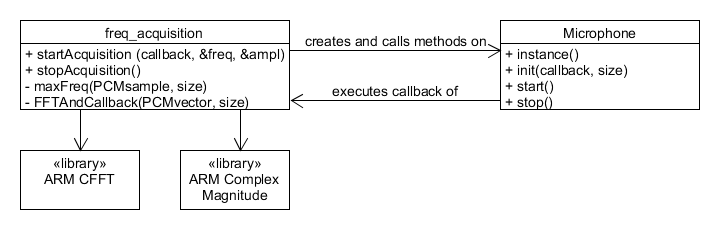
\includegraphics[width= 1.3\textwidth]
	{files/images/freqAcquisitionUML.png}
	\caption{UML schema of the interaction between the modules in frequency recognition.}
\end{figure}


\subsubsection{Usage of the library}
The usage of the library is performed according to these steps:
\begin{enumerate}
	\item Add the \textit{freq\_recognition.cpp} and \textit{freq\_recognition.h} files in the folder of the other source files of the project, and add the \textit{freq\_recognition.cpp} entry in the \textit{SRC} line of the makefile;
	\item Add the \textit{arm\_bitereversal.c}, \textit{arm\_cfft\_radix4\_f32.c}, \textit{arm\_cfft\_radix4\_init\_f32.c} and \textit{arm\_cmplx\_mag\_f32.c} libraries to the project (these libraries are required by \textit{freq\_recognition.cpp});
	\item Add the \textit{\#include "freq\_recognition.h"} line at the start of the source file that will use the library;
	\item Declare 2 float32\_t variables to store the frequency and the amplitude of the last acquired sample;
	\item Define a void callback function without parameters;
	\item Start the acquisition by calling the \textit{startAcquisition(\&callback, \&freq, \&amplitude)} method, passing to it the addresses of the callback function and of the 2 variables. This method is non-blocking (operations are performed in other threads).
\end{enumerate}
Each time a new block of 16-bit PDM samples has been acquired, the driver will perform an FFT analysis on it and will write the frequency and the amplitude of the sample in the chosen variables, then the callback function will be called automatically. This process will be iterated continuously until the \textit{stopAcquisition()} function is called.
\newpage

\subsection{Displaying the recognized frequency}
The transmitter is equipped with a standard HD44780 LCD with two rows and sixteen columns, that is used to print the currently recognized frequency and the associated command (if any).

\subsubsection{Connections}
\begin{tabular}{|c|c|}
	\hline 
	\textbf{LCD pin} & \textbf{Connected to} \\ 
	\hline 
	(1) Vss & GND \\ 
	\hline 
	(2) Vdd & 5V \\ 
	\hline 
	(3) V0 & center tap of a potentiometer between 5V and GND \\ 
	\hline 
	(4) RS & PE7 pin of the Discovery board \\ 
	\hline 
	(5) RW & GND \\ 
	\hline 
	(6) E & PE8 pin of the Discovery board \\ 
	\hline 
	(7) D0 & 5V \\ 
	\hline 
	(8) D1 & 5V \\ 
	\hline 
	(9) D2 & 5V \\ 
	\hline 
	(10) D3 & 5V \\ 
	\hline 
	(11) D4 & PE11 pin of the Discovery board \\ 
	\hline 
	(12) D5 & PE12 pin of the Discovery board \\ 
	\hline 
	(13) D6 & PE13 pin of the Discovery board \\ 
	\hline 
	(14) D7 & PE14 pin of the Discovery board \\ 
	\hline 
	(15) A & 3.3V \\ 
	\hline 
	(16) K & GND \\ 
	\hline 
\end{tabular} 

\subsubsection{Driver and usage}
The driver of the display for Miosix is available in the OS itself: to use it, the \textit{utils/lcd44780.h} library has been included in the main program. \\
	In the software, the display is represented as an instance of the \textit{Lcd44780} class, whose constructor needs to know the pins of the board on which the RS, E, D4, D5, D6, D7 display pins are connected. Through this object, these methods are available:
 \begin{itemize}
 	\item \textit{clear()} to wipe the content of the screen;
 	\item \textit{go(column, row)} moves the cursor to the specified position;
 	\item \textit{printf()} prints to the display, using the standard C formatting rules.
 \end{itemize}

To reduce the risk of printing errors and the required number of updates, the \textit{Lcd44780} instance is encapsulated in an class, named \textit{Display}, in the homonym package. This class exposes only two methods: the first is to set the frequency and the others to set the commands. When one of these are invoked, it will update the display if and only if the passed value is not yet shown.